state estimation to be designed will be deployed in two cars
non-autonomous EV, newly built -> sensors can be chosen
partly autonomous DV, reuse old car with camera/lidar -> fixed set of sensors

\section{Vehicle Characteristics}
car is equipped with a plethora of sensors, but only some are important to us
top down view of car with sensor positions
table: sensor name, sensor type, measured variables, columns EV and dv with X
refer to characterization in TC paper

ES910 as ECU, can be programmed in Matlab/Simulink, C, ASCET-MD~\cite[p.~17]{ETASGmbHStuttgart.2018}
runs \gls{vdc} with TC, TV, motor request...
The VDC is a tool that helps the driver to exploit the maximum physical potential of the vehicle.
state estimation will be part of \gls{vdc}
In DV vehicle, DV software runs on a separate computer that needs part of state as well
inputs from sensor via CAN at different frequencies to avoid congestion
it is unclear whether sfii will be in DV

\section{Requirements}
goal: provide robust, accurate estimate of vehicle state for \gls{vdc} while supporting flexible sensor setups and detecting sensor failures
state variables to estimate
real-time: needs to be computable in 1 ms frequency
complete in all areas, so no developments in near future are necessary

\section{Architecture}
At high level: state estimation = preprocessing + outlier detection + state estimation
To fulfill requirements of robustness and accuracy: outlier detection and sensor fusion
For practical reasons: preprocessing

For flexibility: outlier detection and sensor setup detection using same mechanism
in both cases, sensor cannot or should not be used in sensor fusion
does not matter if not connected, not sending, invalid values

\begin{figure}[h]
	\centering
	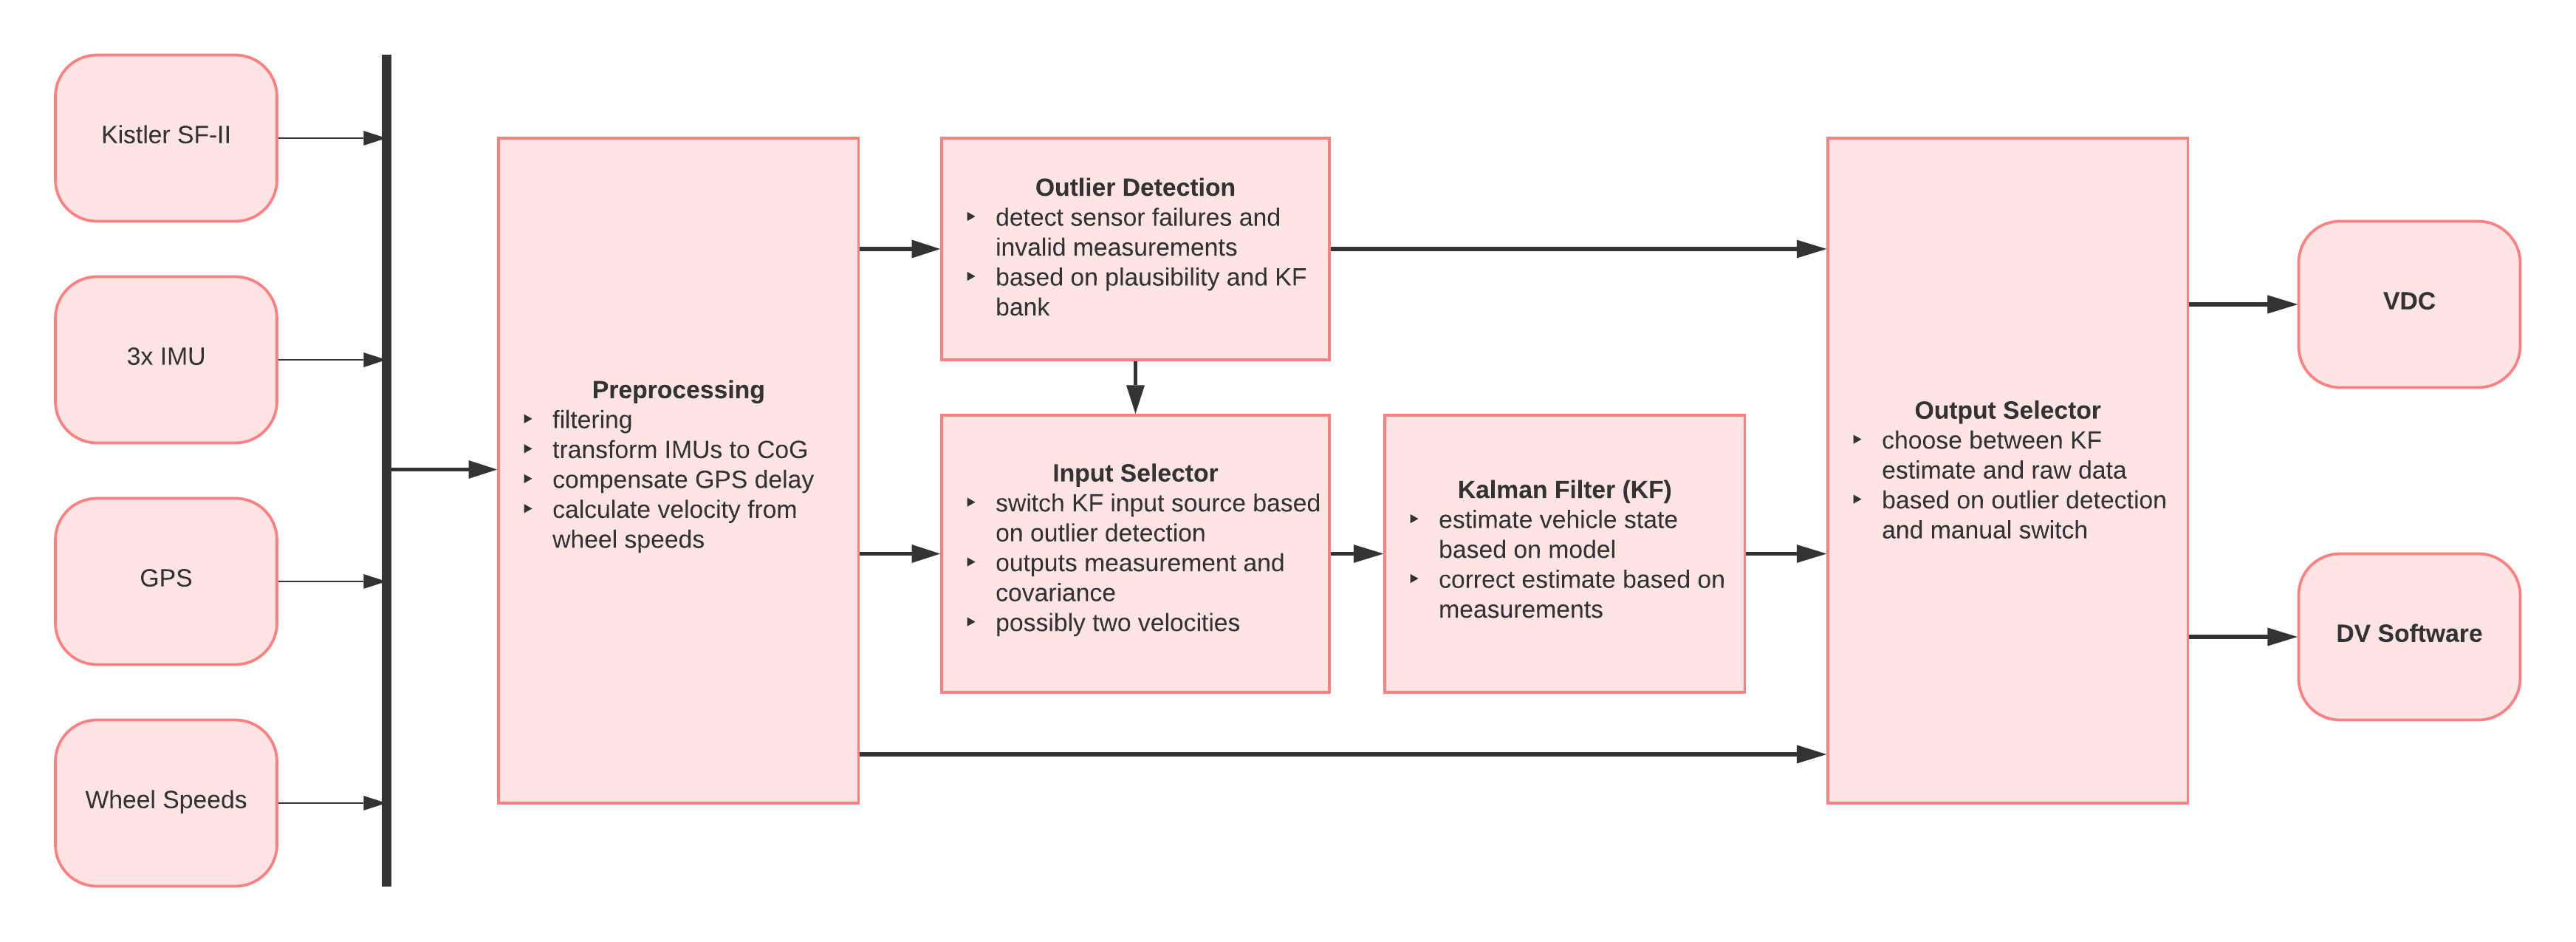
\includegraphics[width=\textwidth]{architecture}%
	\caption{High-level architecture}
	\label{fig:architecture}
\end{figure}

design principle: use simple methods if they work just as well (occam's razor)
easier to understand and troubleshoot
make less assumptions and thus generalize better
only if the results are not adequate, try more complicated approaches

\section{Preprocessing}
convert to SI units so formulas can be applied
show necessary transformations for each measurement
IMU fusion

\section{Outlier Detection}
Show diagram of AND and OR

\section{EKF}
Show input selection and state equations, jacobians
euler forward discretization
